% Código TikZ para tabla de pasos mejorada
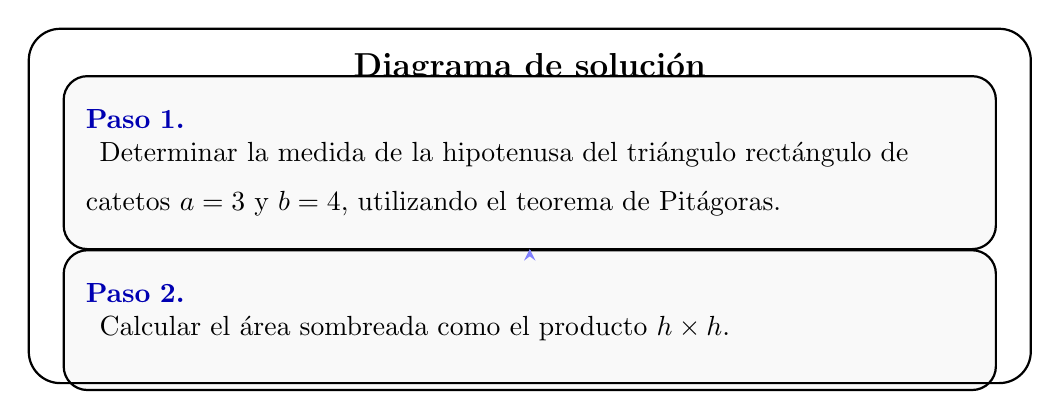
\begin{tikzpicture}[
    box/.style={
        rectangle,
        draw=black,
        thick,
        minimum width=0.95\textwidth,
        text width=0.93\textwidth,
        rounded corners=3mm,
        inner sep=8pt,
        inner ysep=12pt,
        fill=gray!5
    },
    title/.style={
        font=\large\bfseries,
        text=black,
        align=center
    },
    step/.style={
        font=\bfseries,
        text=black!80,
        align=left
    },
    description/.style={
        font=\normalsize,
        text=black,
        align=justify
    }
]

% Título
\node[title] at (0,0) {Diagrama de solución};

% Paso 1
\node[box] (paso1) at (0,-1.2) {
    \begin{minipage}{\linewidth}
        \textcolor{blue!70!black}{\textbf{Paso 1.}} \\
        \vspace{0.2cm}
        Determinar la medida de la hipotenusa del triángulo rectángulo de catetos $a = 3$ y $b = 4$, utilizando el teorema de Pitágoras.
    \end{minipage}
};

% Paso 2
\node[box] (paso2) at (0,-3.2) {
    \begin{minipage}{\linewidth}
        \textcolor{blue!70!black}{\textbf{Paso 2.}} \\
        \vspace{0.2cm}
        Calcular el área sombreada como el producto $h \times h$.
    \end{minipage}
};

% Línea conectora entre pasos
\draw[-stealth, thick, blue!50] (paso1.south) -- (paso2.north);

% Borde exterior
\draw[rounded corners=4mm, black, thick] 
    (-0.5\textwidth-0.3cm, 0.5cm) rectangle 
    (0.5\textwidth+0.3cm, -4.0cm);

\end{tikzpicture}
